\documentclass[12pt]{article}
\usepackage{ctex}
\usepackage[english]{babel}
\usepackage{blindtext}
\usepackage{nameref}
\usepackage{fancyhdr}
\usepackage{amsmath,amssymb,amsthm}
\usepackage{graphicx,float}
\usepackage{physics}
\usepackage{pgfplots}
\usepackage[a4paper, total={6in, 9in}]{geometry}

\graphicspath{{../image/}}

\pagestyle{fancy}
\fancyhf{}
\fancyhf[HL]{微分幾何1:向量與導數}
\fancyhf[CF]{\thepage}

\newcommand{\innerprod}[2]{\langle{#1},{#2}\rangle}
\newcommand{\id}{\mathtt{id}}

\newtheorem{definition}{定義}
\newtheorem*{theorem}{定理}
\newtheorem*{corollary}{衍理}
\newtheorem*{lemma}{引理}
\newtheorem*{proposition}{命題}
\newtheorem*{remark}{小記}
\newtheorem*{claim}{主張}
\newtheorem*{example}{示例}
\newtheorem*{axiom}{公設}
\renewenvironment*{proof}{\textit{證明.}}{\hfill$\qed$}

\newenvironment*{sol}{\par \textbf{解}.}{\hfill$\blacksquare$}

\begin{document}
    References: Introduction to Real Analysis (Bartle \& Sherbert), Thomas Calculus 12th Edition
    \section*{向量}

    向量屬於一種特殊的矩陣,通常用以表達\textbf{多維坐標}。

    \begin{definition}[向量]
        一個\textbf{$n$-維向量}包含$n$個元素,可視之爲\textbf{$n$-維空間}中的坐標,同時代表從原點指向該坐標的箭頭。
    \end{definition}
    
    爲方便描述,記$V_S$為帶有$S$域的元素的向量集合。

    \begin{definition}[向量加法]
        在向量集合$V_S$中,若$\vec{x}=(x_i)_i=(x_1,x_2,\dots),\vec{y}=(y_i)_i=(y_1,y_2,\dots)\in V_S$,則$$\vec{x}+\vec{y}:=(x_1+y_1,x_2+y_2,\dots)=(x_i+y_i)_i$$
    \end{definition}

    \begin{definition}[標量乘法]
        在向量集合$V_S$中,若$\vec{x}=(x_i)_i=(x_1,x_2,\dots)\in V_S$,$\alpha \in S$,則$$\alpha \vec{x}:=(\alpha x_1,\alpha x_2,\dots)=(\alpha x_i)_i$$
    \end{definition}

    \begin{definition}[向量的量值]
        對於任意向量$\vec{v}$,其量值定義爲$|\vec{v}|$,代表其長度。
    \end{definition}
    \section*{向量空間}

    \begin{definition}[向量空間]
        設$V_S$為向量集合,且$\vec{x},\vec{y},\vec{z}\in V_S$, $\alpha, \beta \in S$。若$V_S$符合以下定理:\begin{itemize}
            \item 加法結合律:$(\vec{x}+\vec{y})+\vec{z}=\vec{x}+(\vec{y}+\vec{z})$。
            \item 加法交換律:$\vec{x}+\vec{y}=\vec{y}+\vec{z}$。
            \item 加法單位元:$\vec{0}\in V_S$使得$\vec{x}+\vec{0}=\vec{0}+\vec{x}=\vec{x}$。
            \item 加法逆:$\forall \vec{x}\in V_S$, 存在$\vec{y}\in V_S$使得$\vec{x}+\vec{y}=\vec{y}+\vec{x}=\vec{0}$。
            \item 標乘結合律:$\alpha(\beta \vec{x})=(\alpha\beta)\vec{x}$。
            \item 標乘單位元:$1\in S$使得$1\vec{x}=\vec{x}$。
            \item 分配律1:$\alpha(\vec{x}+\vec{y})=\alpha\vec{x}+\alpha\vec{y}$。
            \item 分配律2:$(\alpha+\beta)\vec{x}=\alpha\vec{x}+\beta\vec{x}$。
        \end{itemize}
    \end{definition}

    \begin{example}
        $\mathbb{R}$是一個向量空間。而且任何域也是向量空間。
    \end{example}

    \begin{example}
        在牛頓力學中討論力時,我們會以向量表示力的大小與方向。假設目前的討論僅限於平面(二維空間),並記施力點為原點$O$。
        \begin{figure}[H]
            \centering
            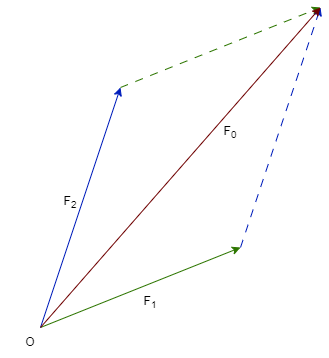
\includegraphics[scale=0.6]{Force.png}
        \end{figure}
        在上圖中可通過改變力量發生的先後次序來實現向量的平移,從而得出$$\vec{F_0}=\vec{F_1}+\vec{F_2}$$的關係式。
        又因二維向量可拆分爲水平向量及鉛垂向量兩個分量,故$$\vec{F_0}=(|\vec{F_1}|\cos{\theta}+|\vec{F_2}|\cos{\phi})\hat{i}+(|\vec{F_1}|\sin{\theta}+|\vec{F_2}|\sin{\phi})\hat{j}$$其中$\hat{i}$和$\hat{j}$分別代表水平單位向量及鉛垂單位向量。
    \end{example}

    欲考慮作功問題,我們定義以下計算方式

    \begin{definition}[點積/内積]
        兩向量$\vec{a},\vec{b}$的内積可定義爲$$\innerprod{\vec{a}}{\vec{b}}\equiv \vec{a}\cdot\vec{b}:=|\vec{a}||\vec{b}|\cos{\theta}$$其中$\theta$為$\vec{a},\vec{b}$之間的夾角。
    \end{definition}

    \begin{example}
        根據經典力學定義,作功方程爲$$W=\vec{F}\cdot\vec{s}$$其中$W$為作功純量,$\vec{F}$為施力向量,$\vec{s}$為位移向量。考慮内積定義,作功方程可寫成$$W=|\vec{F}||\vec{s}|\cos{\theta}$$其中$\theta$為向量之間的夾角。
    \end{example}

    \begin{theorem}[内積的性質]
        對於$\vec{a},\vec{b},\vec{c}$,\begin{enumerate}
            \item $\innerprod{0}{\vec{a}}=\innerprod{\vec{a}}{0}=0$;
            \item $\innerprod{\vec{a}}{\vec{a}}\geq 0$,$\innerprod{\vec{a}}{\vec{a}}=0$當且僅當$\vec{a}\equiv 0$;
            \item $\innerprod{\vec{a}}{x\vec{b}+z\vec{c}}=x\innerprod{\vec{a}}{\vec{b}}+z\innerprod{\vec{a}}{\vec{c}}$;
            \item 若$\vec{a},\vec{b}\in\mathbb{R}^n$,則$\innerprod{\vec{a}}{\vec{b}}=\innerprod{\vec{b}}{\vec{a}}$。
        \end{enumerate}
    \end{theorem}

    \begin{proposition}
        向量$\vec{a},\vec{b}$之間的夾角為$$\theta=\arccos{\frac{\vec{a}\cdot\vec{b}}{|\vec{a}||\vec{b}|}}$$
    \end{proposition}

    另外,若$\vec{a}$正交於$\vec{b}$(在$\mathbb{R}^2$為互相垂直),$\vec{a},\vec{c}$平行,則根據定義$$\vec{a}\cdot\vec{b}=|\vec{a}||\vec{b}|\cos{90^\circ}=0$$及$$\vec{a}\cdot\vec{c}=|\vec{a}||\vec{c}|\cos{0^\circ}=|\vec{a}||\vec{c}|$$
    因此$$|\vec{a}|=\sqrt{|\vec{a}|^2}=\sqrt{\innerprod{\vec{a}}{\vec{a}}}$$
    \begin{definition}[基與正交基與標準正交基]
        對於向量空間$V_S$,若$\{\vec{b_1},\vec{b_2},\dots,\vec{b_n}\}\subset V_S$為互不平行,即綫性獨立,同時對任意$\vec{v}\in V_S$,都存在$\alpha_1,\alpha_2,\dots,\alpha_n\in S$使得$$\vec{v}=\sum_{k=1}^{n}\alpha_k \vec{b_k}$$則稱$\{\vec{b_1},\vec{b_2},\dots,\vec{b_n}\}$為$V_S$的\textbf{基}。

        若$\{\vec{\beta_1},\vec{\beta_2},\dots,\vec{\beta_n}\}\subset V_S$為$V_S$的基而且對所有$i\neq j$,均有$$\innerprod{\vec{\beta_i}}{\vec{\beta_j}}=0$$則稱$\{\vec{\beta_1},\vec{\beta_2},\dots,\vec{\beta_n}\}$為$V_S$的\textbf{正交基}。

        若$\{\vec{\gamma_1},\vec{\gamma_2},\dots,\vec{\gamma_n}\}\subset V_S$為$V_S$的正交基而且對所有$i$,均有$$|\vec{\gamma_i}|=1$$則稱$\{\vec{\gamma_1},\vec{\gamma_2},\dots,\vec{\gamma_n}\}$為$V_S$的\textbf{標準正交基}。
    \end{definition}
    
    \begin{remark}
        對於任何向量空間,標準正交基的構成并非唯一。舉例$\mathbb{R}$作爲$\mathbb{R}$的向量空間,$1$和$-1$均可作爲$\mathbb{R}$的標準正交基;$\mathbb{R}^2$作爲$\mathbb{R}$的向量空間,則$$\{\begin{bmatrix}
            \cos{\theta}\\\sin{\theta}
        \end{bmatrix},\begin{bmatrix}
            -\sin{\theta}\\\cos{\theta}
        \end{bmatrix}:\theta\in\mathbb{R}\}$$均爲$\mathbb{R}^2$的標準正交基。
    \end{remark}

    對於有標準正交基的向量空間,我們的討論會比較簡單:

    \begin{theorem}
        設$V_S$為向量空間,$\{e_1,e_2,\dots,e_n\}$為$V_S$的標準正交基。若$v,u\in V_S$可寫作$v=\sum_{i=1}^{n}v_i e_i$及$u=\sum_{i=1}^{n}u_i e_i$,則$$\innerprod{u}{v}=\sum_{i=1}^{n}u_iv_i$$
    \end{theorem}

    \begin{proof}
        \begin{align*}
            \innerprod{u}{v}
            &=\innerprod{\sum_{i=1}^{n}u_i e_i}{\sum_{j=1}^{n}v_j e_j}
            =\sum_{i=1}^{n}u_i\innerprod{e_i}{\sum_{j=1}^{n}v_j e_j}
            =\sum_{i=1}^{n}\sum_{j=1}^{n}u_iv_j\innerprod{e_i}{e_j}\\
            &=\sum_{i=1}^{n}\sum_{j=1}^{n}u_iv_j\delta_{ij}
            =\sum_{\substack{
                i=j\\1\leq i,j\leq n
            }}u_iv_j
            =\sum_{i=1}^{n}u_iv_i
        \end{align*}
    \end{proof}

    \begin{corollary}
        設$V_S$為向量空間,$\{e_1,e_2,\dots,e_n\}$為$V_S$的標準正交基。若$v\in V_S$可寫作$v=\sum_{i=1}^{n}v_i e_i$,則$$|v|=\sqrt{\sum_{i=1}^{n}v_i^2}$$
    \end{corollary}

    爲方便描述,接下來會稱$V_S$的標準正交基為$\mathcal{O}(V_S):= \{e_i\}_{i\in I}$,$I$為索引集。

    \begin{theorem}[餘弦定理]
        設$u,v\in V_S$,則$$|u-v|^2=|u|^2+|v|^2-2|u||v|\cos{\theta}$$其中$\theta$是$u,v$的夾角。
    \end{theorem}

    \begin{proof}
        設$u=\sum_{i\in I}u_ie_i, v=\sum_{i\in I}v_ie_i$,則\begin{align*}
            |u-v|^2&=\sum_{i\in I}(u_i-v_i)^2\\
            &=\sum_{i\in I}(u_i^2+v_i^2-2u_iv_i)\\
            &=\sum_{i\in I}u_i^2+\sum_{i\in I}v_i^2-2\sum_{i\in I}u_iv_i\\
            &=|u|^2+|v|^2-2\innerprod{u}{v}\\
            &=|u|^2+|v|^2-2|u||v|\cos{\theta}
        \end{align*}
    \end{proof}

    在三維空間中,存在外積:

    \begin{definition}[外積]
        假設$\{\hat{i},\hat{j},\hat{k}\}\subset \mathbb{R}^3$為$\mathbb{R}^3$的標準正交基,則定義$\times:\mathbb{R}^3\to\mathbb{R}^3$為$$\hat{i}\times \hat{j}=\hat{k},\hat{j}\times \hat{k}=\hat{i}, \hat{k}\times \hat{i}=\hat{j}$$
    \end{definition}

    外積的定義可考慮面積與體積的計算原理:考慮三個單位向量$\hat{i},\hat{j},\hat{k}$的乘積為體積及任意兩個向量的乘積為面積,基於$\hat{i}\times \hat{j}$為$ij$平面的面積單位,而面積乘以高等於體積,故$V(\hat{i},\hat{j},\hat{k})=(\hat{i}\times \hat{j})\cdot \hat{k}$為標量,使得$\hat{i}\times\hat{j}=\hat{k}$。

    因此,我們可定義

    \begin{definition}[面積與體積]
        設$u,v,w\in\mathbb{R}^3$,則\begin{align*}
            A(u,v)&:=|u\times v|=\left|\left|\begin{matrix}
                \hat{i}&\hat{j}&\hat{k}\\
                u_1&u_2&u_3\\
                v_1&v_2&v_3
            \end{matrix}\right|\right|\\
            V(u,v,w)&:=(u\times v)\cdot w=\left|\begin{matrix}
                u_1&u_2&u_3\\
                v_1&v_2&v_3\\
                w_1&w_2&w_3
            \end{matrix}\right|\\
        \end{align*}
    \end{definition}

    \section*{向量函數}

    \section*{偏導數與全導數}

    \section*{方向導數}

    \section*{切面與法綫}

    \section*{二維極值與鞍點}
\end{document}